%% Based on a TeXnicCenter-Template by Tino Weinkauf.
%%%%%%%%%%%	%%%%%%%%%%%%%%%%%%%%%%%%%%%%%%%%%%%%%%%%%%%%%%%%%%

%%%%%%%%%%%%%%%%%%%%%%%%%%%%%%%%%%%%%%%%%%%%%%%%%%%%%%%%%%%%%
%% HEADER
%%%%%%%%%%%%%%%%%%%%%%%%%%%%%%%%%%%%%%%%%%%%%%%%%%%%%%%%%%%%%
\documentclass[letterpaper,twoside,12pt]{article}
% Alternative Options:
%	Paper Size: a4paper / a5paper / b5paper / letterpaper / legalpaper / executivepaper
% Duplex: oneside / twoside
% Base Font Size: 10pt / 11pt / 12pt


%% Language %%%%%%%%%%%%%%%%%%%%%%%%%%%%%%%%%%%%%%%%%%%%%%%%%
\usepackage[USenglish]{babel} %francais, polish, spanish, ...
\usepackage[T1]{fontenc}
\usepackage[ansinew]{inputenc}

\usepackage{lmodern} %Type1-font for non-english texts and characters


%% Packages for Graphics & Figures %%%%%%%%%%%%%%%%%%%%%%%%%%
\usepackage{graphicx} %%For loading graphic files
%\usepackage{subfig} %%Subfigures inside a figure
%\usepackage{pst-all} %%PSTricks - not useable with pdfLaTeX

%% Please note:
%% Images can be included using \includegraphics{Dateiname}
%% resp. using the dialog in the Insert menu.
%% 
%% The mode "LaTeX => PDF" allows the following formats:
%%   .jpg  .png  .pdf  .mps
%% 
%% The modes "LaTeX => DVI", "LaTeX => PS" und "LaTeX => PS => PDF"
%% allow the following formats:
%%   .eps  .ps  .bmp  .pict  .pntg


%% Math Packages %%%%%%%%%%%%%%%%%%%%%%%%%%%%%%%%%%%%%%%%%%%%
\usepackage{amsmath}
\usepackage{amsthm}
\usepackage{amsfonts}


%% Line Spacing %%%%%%%%%%%%%%%%%%%%%%%%%%%%%%%%%%%%%%%%%%%%%
%\usepackage{setspace}
%\singlespacing        %% 1-spacing (default)
%\onehalfspacing       %% 1,5-spacing
%\doublespacing        %% 2-spacing


%% Other Packages %%%%%%%%%%%%%%%%%%%%%%%%%%%%%%%%%%%%%%%%%%%
%\usepackage{a4wide} %%Smaller margins = more text per page.
%\usepackage{fancyhdr} %%Fancy headings
%\usepackage{longtable} %%For tables, that exceed one page


%%%%%%%%%%%%%%%%%%%%%%%%%%%%%%%%%%%%%%%%%%%%%%%%%%%%%%%%%%%%%
%% Remarks
%%%%%%%%%%%%%%%%%%%%%%%%%%%%%%%%%%%%%%%%%%%%%%%%%%%%%%%%%%%%%
%
% TODO:
% 1. Edit the used packages and their options (see above).
% 2. If you want, add a BibTeX-File to the project
%    (e.g., 'literature.bib').
% 3. Happy TeXing!
%
%%%%%%%%%%%%%%%%%%%%%%%%%%%%%%%%%%%%%%%%%%%%%%%%%%%%%%%%%%%%%

%%%%%%%%%%%%%%%%%%%%%%%%%%%%%%%%%%%%%%%%%%%%%%%%%%%%%%%%%%%%%
%% Options / Modifications
%%%%%%%%%%%%%%%%%%%%%%%%%%%%%%%%%%%%%%%%%%%%%%%%%%%%%%%%%%%%%

%\input{options} %You need a file 'options.tex' for this
%% ==> TeXnicCenter supplies some possible option files
%% ==> with its templates (File | New from Template...).



%%%%%%%%%%%%%%%%%%%%%%%%%%%%%%%%%%%%%%%%%%%%%%%%%%%%%%%%%%%%%
%% DOCUMENT
%%%%%%%%%%%%%%%%%%%%%%%%%%%%%%%%%%%%%%%%%%%%%%%%%%%%%%%%%%%%%

\usepackage[margin=.9in]{geometry}
\usepackage{natbib}
\usepackage{braket}
\usepackage{titling}

	\setlength{\droptitle}{-8em}
\linespread{1.5}

\newcommand{\ketbra}[1]{|#1\rangle\langle#1|}
\begin{document}

\pagestyle{empty} %No headings for the first pages.


%% Title Page %%%%%%%%%%%%%%%%%%%%%%%%%%%%%%%%%%%%%%%%%%%%%%%
%% ==> Write your text here or include other files.

%% The simple version:
\title{QIC 750 Term Paper - Wigner State Tomography}
\author{John Rinehart}
%\date{} %%If commented, the current date is used.
\maketitle	

%% The nice version:
%\input{titlepage} %%You need a file 'titlepage.tex' for this.
%% ==> TeXnicCenter supplies a possible titlepage file
%% ==> with its templates (File | New from Template...).


%% Inhaltsverzeichnis %%%%%%%%%%%%%%%%%%%%%%%%%%%%%%%%%%%%%%%
\pagestyle{plain} %Now display headings: headings / fancy / ...

%% Chapters %%%%%%%%%%%%%%%%%%%%%%%%%%%%%%%%%%%%%%%%%%%%%%%%%
%% ==> Write your text here or include other files.
\section{Introduction}
\section*{Introduction}
\addcontentsline{toc}{section}{Motivation}
Filters are an important part of the RF/Microwave signal chain. They can be used
to prevent aliasing of signals used with nonlinear devices (like mixers) and
also to prevent interference from signals with proximal frequency components.
Ever filter is qualified by a number of metrics: insertion loss, rejection,
selectivity, group delay, etc. The topology, number and quality of components
determines the filter's behavior and, as such, must be chosen very carefully.

To add to the filter designer's struggles, it can be shown that it is not
possible to design a filter with arbitrarily large bandwidth and arbitrarily high
gain. The derivation of the gain-bandwidth theorem can be found in reference
\cite{wcd}. Thus, it is up to the designer to push the gain-bandwidth
limits to the limit. This requires high-fidelity components and an optimal
design scheme. Material science and component design is under active research.
This will improve the reliability and performance of the components, themselves.

What is needed, then, is to consider a methodology with which the proper
components for an optimal filter design can be considered. The simplified real
frequency technique (SRFT), devised in 1982 by Herbert Carlin and Binboga Yarman
addresses this problem \cite{srft}. Essentially, the SRFT achieves an optimal
filter design by using computer-aided optimization. This report will describe
SRFT and a MATLAB\textsuperscript{\textregistered} implementation of the SRFT
currently under development. The goal of this report is to demonstrate the
efficacy of the SRFT and a particular microwave design which was implement using
the aformentioned MATLAB\textsuperscript{\textregistered} implementation.
 %You need a file 'intro.tex' for this.
\section{Theory}
\section*{Theory}
\addcontentsline{toc}{section}{Theory}

The theory behind the SRFT is simple and relies on 4 basic ideas:

\begin{enumerate}
    \item Optimization of Transducer Gain
    \item Kramers-Kronig Relations
    \item The Gewertz Method
    \item Darlington Synthesis (Pole Extraction at Infinity)
\end{enumerate}

\subsection*{Optimization of Transducer Gain}
\addcontentsline{toc}{subsection}{Optimization of Transducer Gain}

The concept of transducer gain optimization is simple: Consider the source and
the load and allow the introduction of some network that maximizes the power
transfer from the source to the lead. This power transfer will be maximum when
the source and the load are conjugately matched. Thus, the problem can be stated
as follows:

\[
\min_{\text{networks}} \left| \left| T_{\text{goal}}(\omega) -
T_{\text{network}}(\omega) \right| \right|
\]

The idea, stated above, is to declare some goal transducer gain function (that may be
physically impossible based on gain-bandwidth considerations). Then, considering
all possible networks, we minimize over the norm of the difference between the
two transducer gain functions. However, we need some way in which to perform
this minimization. So, we next express the transducer gain of the network in
terms of the impedance of the network and the load:

\[ 
T(\omega) = \frac{4 r R}{(x + X)^2 + (r + R)^2} 
\]

Where, above, lower case $r$ and $x$ indicate load quantities and $R$ and $X$
represent network quantities. It should be clear from this description that the
frequency dependence is captured by all of the four circuit quantities: $r, R,
x, X$. It is precisely this frequency dependence that determines the transducer
gain. It should also be noted that the gain appears to be maximized when the
reactance of the load is cancelled by the reactance of the introduced network.
This is a restatement of the conjugate matching principle stated earlier. Now,
for the purposes of this report, the load will always be considered fixed. The
network is introduce in the context of the load and the transducer gain is
maximized.

They way in which SRFT attempts to determine the optimum resistance
characteristic is determined by the relationship between the resistance and
reactance characteristic and will be discussed subsequently.

\subsection*{Kramers-Kronig Relations}
\addcontentsline{toc}{subsection}{Kramers-Kronig Relations}

A really interesting side-effect of having access to a linear, causal system is
that the real and imaginary parts of the transfer function of such a system are
not independent. It can be shown that the relationship between the real and
imaginary parts of a circuit network $R$ and $X$ are as follows (see \cite{wcd}):


\begin{align*}
    R(\omega) &= - \frac{2}{\pi} \int_{0}^{\infty} \frac{\Omega~X(\Omega)}{\Omega^2 -
\omega^2} d\Omega \\
    X(\omega) &= \frac{2\omega}{\pi} \int_{0}^{\infty}
\frac{R(\Omega)}{\Omega^2-\omega^2} d \Omega
\end{align*}

These are known as the Kramers-Kronig relations. It is at this point that the
numerical optimization procedure is introduced.  Imagine that the resistance as
a function of frequency is broken up into many piecewise segments. Then, for
each break frequency $\omega_k$ there exists some resistance $R_k$ at that break
frequency. $R(\omega)$ can now be expressed as:

\[ 
R(\omega) = R_0 + \sum^{n}_{k=1} D_k a_k(\omega) 
\]

where 

\begin{align*}
    a_k(\omega) =&
    \begin{cases}
        1 & \omega \ge \omega_k \\
        \frac{\omega - \omega_{k-1}}{\omega_k - \omega_{k-1}} &\omega_{k-1} \le
        \omega \le \omega_k \\
        0 &\omega < \omega_{k-1}
    \end{cases}
\end{align*}

It is clear from this, then, that $D_k$ represents the slope of the kth break
frequency and, as such:

\[ 
D_k = R_k - R_{k-1} 
\]

If this is the form of $R(\omega)$ that is assumed for the SRFT then it can be
shown that the reactance must be related to $R(\omega)$ by:

\[
X(\omega) = \sum^{n}_{k=1} D_k b_k(\omega)
\]

where
\begin{align*}
    b_k(\omega) = (\pi \left( \omega - \omega_{k-1} \right))^{-1} \big(
&\left( \omega + \omega_k \right) \ln \left| \omega + \omega_k \right| +
\\
&\left( \omega - \omega_k \right) \ln \left| \omega - \omega_k \right| - \\
&\left(\omega + \omega_{k-1} \right) \ln \left| \omega + \omega_{k-1} \right| - 
\\
&\left( \omega - \omega_{k-1} \right) \ln \left| \omega - \omega_{k-1} \right| 
\big)
\end{align*}

This expression for $X(\omega)$ is nothing more than the previous expressions
relating $R(\omega)$ to $X(\omega)$ assuming that $R(\omega)$ has a piecewise
linear form. This piecewise linearity makes it easy to calculate the reactance
on a computer. Since the goal is to reduce the difference between the goal gain
function and the network gain function, the algorithm will perform the
following: It will adjust the $D_k$s using some scheme (gradient ascent, random,
etc.) and will attempt to produce a set of $D_k$s that makes the difference
between $T_{network}$ and $T_{goal}$ a minimum. Those $D_k$s will correspond to
some $R(\omega)$ and some $X(\omega)$. Thus, it would seem that the $D_k$
correspond to some network. It is this point that we have to introduce the way
in which the network is deduced from $R(\omega)$ and $X(\omega)$.

\subsection*{The Gewertz Method}
\addcontentsline{toc}{subsection}{The Gewertz Method}

In order to determine a network from the obtained piecewise linear $R(\omega)$,
I can perform the following. It can be shown that the impedance of the network
and the resistance of the network are related:

\[ 
R(-s^2) = \frac{1}{2} \left( Z(s) + Z(-s) \right) 
\]

where $s = j\omega$. The reason for expression $R$ as a function of $s^2$ is
that the resistance function must be even about $\omega = 0$, by physical
considerations. So, now, consider that the piecewise linear $R(\omega)$ is
approximated by some rational function fit $\tilde{R}(-s^2) =
\frac{p(-s^2)}{q(-s^2)}$.  Now, consider $Z(s) = \frac{n(s)}{d(s)}$, where $n$
and $d$ are the numerator and denominator polynomials of $Z(s)$, respectively.
It can be shown, then, that by relating the coefficients of $p(-s^2)$ with those
of $d(s)$ and $n(s)$ that the following holds (note that $d(s)d(-s) = q(-s^2)$):

\[ 
    \begin{pmatrix} p_0 \\ p_2 \\ \vdots \\ p_{2m} \end{pmatrix} = 
        \begin{pmatrix}
            d_0 & 0    & \ldots & 0 & 0      \\
            d_2 & -d_1 & \ldots & 0 & 0      \\
            \vdots & \vdots & \vdots & \vdots & \vdots \\
            0   &   0  & \ldots & -d_{m-1} & d_{m-2} \\
            0   &   0  & \ldots & 0 & d_{m} 
        \end{pmatrix}
        \begin{pmatrix}
            n_0 \\ n_1 \\ \vdots \\ n_{m-1} \\ n_{m}
        \end{pmatrix}
\]

Above, it is assumed that $p(s) = \sum^{2m-2}_{i=1} p_i s^i$ and similarly with
the other polynomials.

Now, our goal is to solve for $Z(s) = \frac{n(s)}{d(s)}$. We can obtain the
coefficients of $d(s)$ from those of $q(s)$ (we have $q(-s^2)$ from our fit of
$R(-s^2)$) by using spectral factorization. According to \cite{wcd}, any
real non-negative function $A(-s^2)$ can be written as a product, $a_0^2
a(s)a(-s)$, where $a_0$ is real and $a(s)$ is a real monic polynomial. Thus, we
know the coefficients $d_0, d_1, d_2,\ldots, d_{2m}$ which form $d(s)$ since we
know $q(-s^2)$ from having had fit $R(s)$ to a rational function.

We can then invert the above equation to find the numerator polynomial
coefficients. Once we have $n(s)$ from the aforementioned procedure, we form
$Z(s) = \frac{n(s)}{d(s)}$. This is the Gewertz method.

What we need now is a way in which to obtain the network (resistors, inductors,
capacitors) from $Z(s)$. This is what Darlington synthesis enables us to do.

\subsection*{Darlington Synthesis}
\addcontentsline{toc}{subsection}{Darlington Sythesis}

It is shown in reference \cite{wcd} that any realizable impedance function can
be realized as a lossless LC ladder network terminated on a resistor. The proof
will not be given here but a demonstration of the technique will be described.
Assuming that $Z(s)$ is expressed as a rational function (which can always be
done to at least some approximation), then the network can be constructed as
follows:

\[ 
Z(s) = \frac{n_0 + n_1 s + n_2 s^2 + \ldots + n_m s^m}{d_0 + d_1 s + d_2 s^2 +
\ldots + d_m s^m} 
\]

Then, by iterative division, $Z(s)$ can be expressed as a continued fraction:

\[ 
Z(s) = \frac{1}{\frac{d_0 + d_1 s + d_2 s^2 +
\ldots + d_m s^m}{n_0 + n_1 s + n_2 s^2 + \ldots + n_m s^m}} 
\]

Then, using long division, this can be expressed in the form:

\[
Z(s) = \frac{1}{c_0(s) + \frac{1}{c_1(s) + \frac{1}{c_2(s) + \ldots}}}
\]

Now, this is exactly the form of an LC ladder network input impedance. By
construction, $c_0(s)$ is at most a first order polynomial in $s$. This holds
true for other $c_i(s)$ also. Consider the case, for example, when $c_0(s) =
.5s$. This is exactly a capactive admittance of value
\SI[parse-numbers=false]{.5s}{\siemens} which corresponds to a capacitance of
\SI{.5}{\farad}. Thus, the first element in the network would be a shunt
capacitance (since it's an admittance) of \SI{.5}{\farad}. So, apparently,
expressing the impedance in this form by repeating iterative long division is a
way in which the components of the network are made easily visible.

Once the components are identified, all that remains is to simulate the network
determined by the algorithm to ensure that it, indeed, satisfies the properties
desired by the designer; that is, that it approximates well the optimal
gain-bandwidth characteristic.

Now that the theory has been established, a practical example of a filter will
be undertaken and the network will by synthesized and simulated. The
shortcomings of the current implementation will be discussed subsequently.


\section{Smithey et. al.}
In 1993 Smithey et. al. reported making an experimental determination of a single-mode of the vacuum state's electrical field \cite{Smithey}. In addition to making a bare measurement of the electrical field they, also, measured a squeezed state of the vacuum electrical field. Note that their approach was optical and that they used a slightly different form of the Wigner function than is proposed by Leonhardt (given earlier) : $W(x,p)=\frac{1}{\pi}\int\limits_{-\infty}^{\infty}\bra{x+x'}\rho\ket{x-x'}e^{-2ipx'}dx'$.

\begin{figure}%
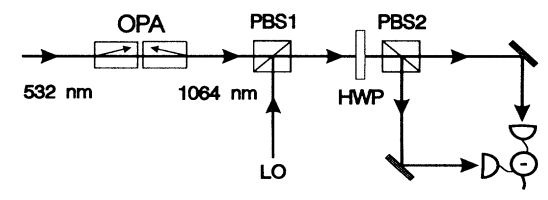
\includegraphics[width=274px,height=100px]{Figures/SmitheySetup.png}%
\caption{Experimental set-up as reported in \cite{Smithey}. An optical parametric amplifier is driven to upconvert a 532 nanometer signal to a 1064 nanometer signal. In the case of the measurement of squeezed radiation, the output of the parametric amplifier is one of the two inputs to a single port of a 50-50 (balanced) polarizing beam splitter, PBS1 - the other input being the local oscillator (whose association with a piezoelectric crystal determines the phase relationship between the signal and the local oscillator). In the case of the measurement of unsqueezed radiation the output of the parametric amplifier is blocked; then the non-LO input to PBS1 is simply the vacuum state. The polarization of the light into the second polarizing beam splitter, PBS2, adjusted with a $\frac{\lambda}{2}$ plate (HWP).  The effect of the half-wave plate is to rotate components of the polarization by $45^\circ$. The placement of the last beam splitter produces a superposition of the two incident beams (the vacuum and the combined signal from the first beam splitter). The two superposition beams are detected by the two photodetectors. The two output signals are then processed and analyzed to obtain the quadrature probability distributions, $P_\phi(x_\phi)$.}
\label{SmitheySetup}%
\end{figure}

Experimentally, their set-up was as is shown in Figure \ref{SmitheySetup}. The phase between the local oscillator and the input signal is controlled by the position of a piezoelectric mirror. The piezoelectric mirror allows for modulation of the beam's path length over fractions of a wavelength. The intensity of the two beams is subtracted and the intensity of the difference is directly proportional to the position operator ($x_\phi$) of the signal. Thus, sweeping the position of the piezoelectric mirror over a measurement of the difference of the intensities between the two photodiodes (photodetectors) determines the probability distribution of $x_\phi$ ($P_\phi(x_\phi)$) The phase (the piezoelectric mirror) was varied over 27 distinct positions (phases) and the intensities measured were histogrammed into 64 bins. This analysis, coupled with the aforedescribed measurement process, yielded the probability distribution explained in Figure \ref{SPDR}.

Their experiment is notable due to its historical weight. Smithey et. al. were the first to perform such a Wigner characterization of a quantum mechanical state. At the time, this was fairly novel. It did not gain much popularity and did not see considerable development for ~10 years (until Banaszek et. al. performed their direct Wigner tomography).

\begin{figure}%
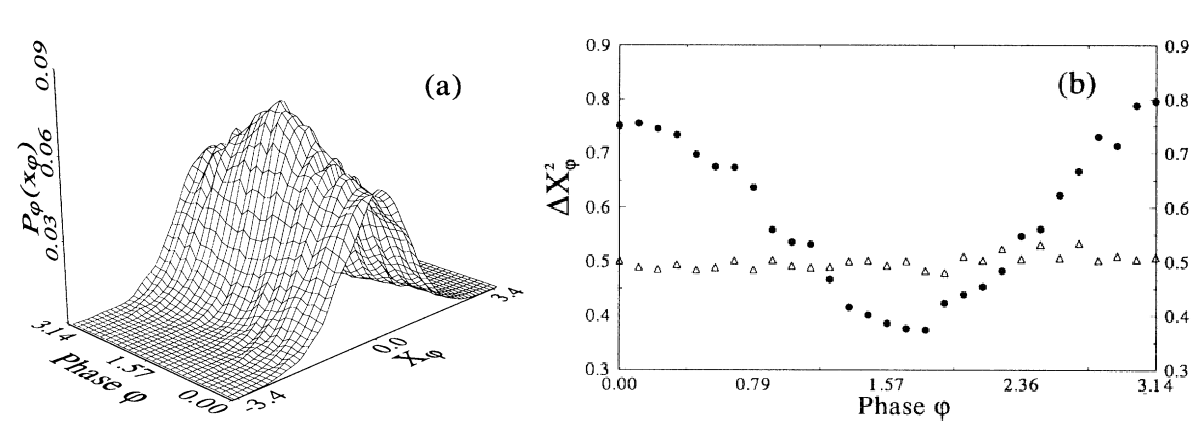
\includegraphics[width=350px,height=138px]{Figures/SmitheyProbabilityDistributionResults.png}%
\caption{Experimental data obtained by Smithey et. al. Show in a) is the marginal distribution of $x_\phi$, of $P_\phi{x_\phi,p_\phi}$, as a function of the local oscillators' swept phase. Panel b) shows the fluctuations of the position quadrature as a function of the local oscillator phase. The near-constant value of .5 for the triangular markers is indicative of vacuum fluctuations (whose variance is constant over the parameter space formed by $x_\phi$ and $p_\phi$). Similarly, the sinusoidal variation of the fluctuations in $x_\phi$, exemplified by the circular markers, is indicative of quadrature squeezing of the vacuum field. Portions of the data which fall significantly below .5 are indicative of the squeezing of the position quadrature. Portions of the data which lie significantly above .5 indicate squeezing of the momentum quadrature.}%
\label{SPDR}%
\end{figure}

\section{Del\'{e}glise et. al.}
In 2008, Del\'{e}glise et. al. \cite{Deleglise} performed markedly different state preparation and characterization compared to that done by Smithey et. al \cite{Smithey}. Their approach involved the use of a cavity quantum electrodynamics (QED) set-up. To prepare the initial state, a highly reflective mirror is brought to superconducting temperatures. The purpose of the mirror is to trap incident photons. One of the purposes of the low temperature for the mirror is to suppress spurious photons generated by the vacuum (which occurs with higher probablility - read: frequency - at higher temperatures. Their scheme purportedly traps the incident light between the mirrors for long times ($130 ms$). A stream of rubidium atoms are prepared such that the state of the atoms (rather the valence electrons) occupy the $n=50$ spherical orbital. The adjacent transition in this atom is the $n=51$ spherical orbital. These serve as the ground and first excited states.

The effect of the cavity field, C in figure \ref{DelSetUp}, on the stream of rubidium atoms is determined by a measurement of the field after the atom is determined to be in the ground or excited state (at D in figure \ref{DelSetUp}). Then, after the state of the atoms (whose state has been modified by the various fields) has been measured a sufficient number of times (millions) the density matrix for the field can be determined. The density matrix obtained for a variety of prepared states is show in figure \ref{DelMeasurements}. The focus of this paper was on the preparation of Schr\"odinger cat states, which are of the form : $|A|(\ket{\alpha}\pm\ket{-\alpha})$, where $|A|$ is the normalization constant and $\ket{\alpha}$ is the conventional notation for a coherent state of light. The reader is reminded that a coherent state of light is one that is expressed in the Fock (number) basis as : $\ket{a} = \sum_{n=0}^{\infty} e^{-\frac{1}{2}\alpha\alpha^*}\frac{\alpha^n}{\sqrt{n!}}\ket{n}=e^{-\frac{1}{2}\alpha\alpha^*}e^{\alpha\hat{a}^\dagger}\ket{0}$. The even cat states and the odd cat states are physically interesting in that an even cat state contains only Fock states of even value while an odd cat state contains only Fock states of odd value.

\begin{figure}%
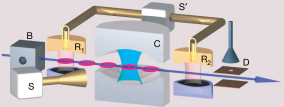
\includegraphics[width=284px,height=107px]{Figures/DelegliseSetUp.png}%
\caption{Cartoon of the experimental set-up used by Del\'{e}glise et. al. The Rydberg atoms (rubidium) are reported as being prepared in `Box B'. These are collimated from the exit port of Box B and projected through the cavity resonator at a speed of 250 $\frac{m}{s}$. Note that, though, there are two cavities external to the main central cavity, C. These cavities $R_1$ and $R_2$ are both used along with an external electromagnetic source (microwave) to prepare the Rydberg atoms in superposition states $\frac{1}{\sqrt{2}}\big(\ket{0}+e^{i\phi}\ket{1}\big)$. The state of the atoms once they have traveled through the three cavity resonators (and having been irradiated three separate times) is determined by the atomic detector, D. Note that the insets have been generated by taking the experimental nonlinearaties of the apparatuses into account.}
\label{DelSetUp}
\end{figure}

Now, while the state preparation is not explained in great detail, the authors of the Del\'eglise paper indicate that the state of the atom upon exiting the third cavity is a linear combination of an even photonic cat state and odd cat state. The even cat state is entangled with the ground state of the rubidium atom and the odd cat state is entangled with the excited state of the rubidium atom. Thus, detector D, which discriminates between excited and ground states of the rubidium atom, projects the state of the field onto one of the Schr\"odinger cat states. If the atom is detected without using detector D to measure the excitation of the atom, the state of the atom entangled to the coherent light in the resonator is, in this case, a statistical mixture of an even and odd cat state. Note that the measured quantity is the radiation escaping from cavity C (not the state of the atoms). The atoms are just used for projective purposes.

The tomography of the states is done in such a way as to, initially, obtain the density matrix of the system. Then, the Wigner function over the phase space (the real and imaginary parts of the field amplitude $\alpha$) is given by $W(\alpha)=\frac{2}{\pi}Tr[D(-\alpha)\rho D(\alpha)e^{i\pi N}]$, where the $N$ in the exponential is the standard bosonic number operator $N = a^\dagger a$. For obvious reasons, this exponentiated operator is often called the parity operator and has eigenvalues $(-1)^n$ (where n is the nth Fock state). The authors make note that the Wigner function would be experimentally determined if the ``atom-field phase shift'' was linear. I understand this to mean than nonlinearities in the mechanisms used to correlate the state of the atom (qubit) to that of the light make a direct determination of the Wigner function impossible. The results of measurement, post-processed, are shown in figure \ref{DelMeasurements}. The density matrices are not shown out of their irrelevance to this paper.

%As a minor addendum	 to the paper, the authors note the significance of the cat states to the study of decoherence. However, the necessity of using cat states (as opposed to any other special quantum state, was not justified.

\begin{figure}%
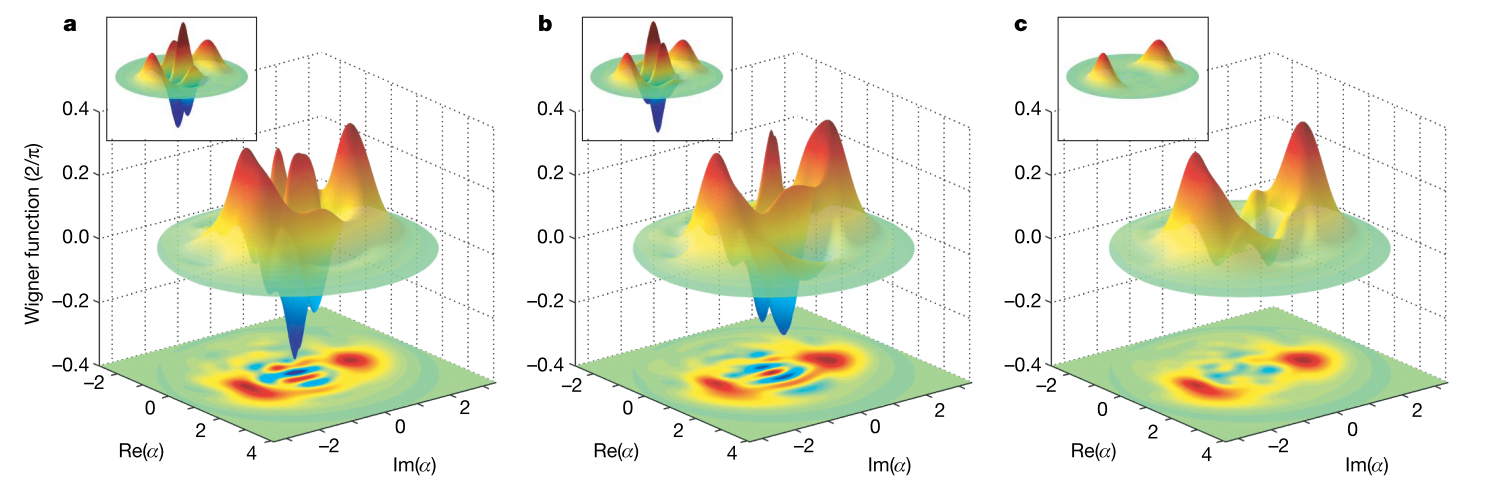
\includegraphics[width=440px,height=149px]{Figures/DelMeasurements.png}%
\caption{Shown in panels a), b) and c) are Wigner function reconstructions for three different states: a) An even Schr\"odinger cat state, b) an odd Schr\"odinger cat stat and c) a symmetric mixture of the even and odd cat states. The theoretically-predicted Wigner function for each respective state is given in the inset of each panel.}%
\label{DelMeasurements}%
\end{figure}



\section{Banaszek et. al.}
In 1999, Banaszek et. al. made direct optical measurements on a number of optical quantum states. Their experimental set-up was fairly simple and the post-processing on their acquired data was relatively trivial. The set-up for their experiment is shown in figure \ref{BanaSetUp}. Typically, the method to determine the Wigner function for a quantum state is to, first, determine the density matrix representation of the state and, second, using the equivalence between the density matrix and the Wigner function, transform the data into the Wigner state-space representation. There are a number of reasons this is typically done. However, the inversion that is needed to go from the discrete density matrix representation to the continuous state-space representation is non-trivial. It typically involves heavy statistics (maximum likelihood estimation theorems to determine which state the data represents) and awkward filtered back-projection schemes analogous to those used in the medical field to render images of the human body using tomography machines (PET, CT, MRI, etc.). There is no utility to this process since the density matrix is the fundamental data set and has just as much information as the Wigner representation.

\begin{figure}%
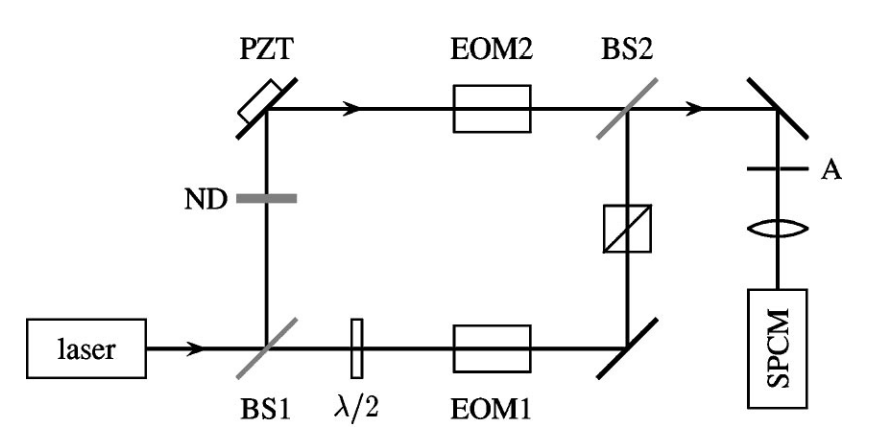
\includegraphics[width=300px,height=153px]{Figures/BanaSetUp.png}%
\caption{Set-up of the optical experiment conducted by Banaszek et. al. in 1999.}%
\label{BanaSetUp}%
\end{figure}

However, Banaszek et. al. implemented a direct measurement of the Wigner function of the quantum state of optical light. The key to sidestepping all the statistics is to realize that the Wigner representation of the state of light (expressed in terms of the displacement of the amplitude of light in phase space) is given by: $W(\alpha)=\frac{2}{\pi}Tr[D(-\alpha)\rho D(\alpha)e^{i\pi N}]$ \cite{Deleglise} which Banaszek et. al. express, equivalently, as  $W(\alpha)=\frac{2}{\pi}\sum_{n=0}^{\infty}(-1)^n D(\alpha)\ket{n}\bra{n} D^\dagger(\alpha)$. Thus, by sweeping $\alpha$ (the phase space parameter), and projecting the resulting quantum state onto the Fock basis, one can determine $W(\alpha)$. Physically, Banaszek et. al. implemented a sweep of $\alpha=|\alpha|e^{i\theta}$ through the use the two branches of their Mach-Zehnder interferometer: a half-wave plate, a Pockels cell (which is a tunable wave plate, called EOM2) and a polarizer control the magnitude of $\alpha=$, $|\alpha|$, while the upper branch, consisting of a neutral density filter (ND) and an electro-optic phase modulator (EOM2) controls the angle of $\alpha$, $\theta$, in phase space; see figure \ref{BanaSetUp}. The measurement of the light is done with a single photon counting module (SPCM). This projects the state of light onto the Fock basis. The piezoelectric translator (piezoelectric mirror, called PZT) is used only for one data set. For this data set, the translator is modulated with a high-frequncy drive, altering the phase of $\alpha$ over very short time scales. In a similar manner as Smithey et. al. \cite{Smithey}, Banaszek et. al. adjusted the amplitude and phase of $\alpha$ in discrete amounts: they used 20 amplitudes and 40 phases of $\alpha$. Many trials are conducted at a particular amplitude and phase, $\alpha_i$ to obtain a distribution over Fock states. Then, $W(\alpha_i)$ is determined. Then, the phase and/or amplitude is adjusted and another multitude of measurements is made. The results of their experiment are shown in figure \ref{BanaResults}.



\begin{figure}%
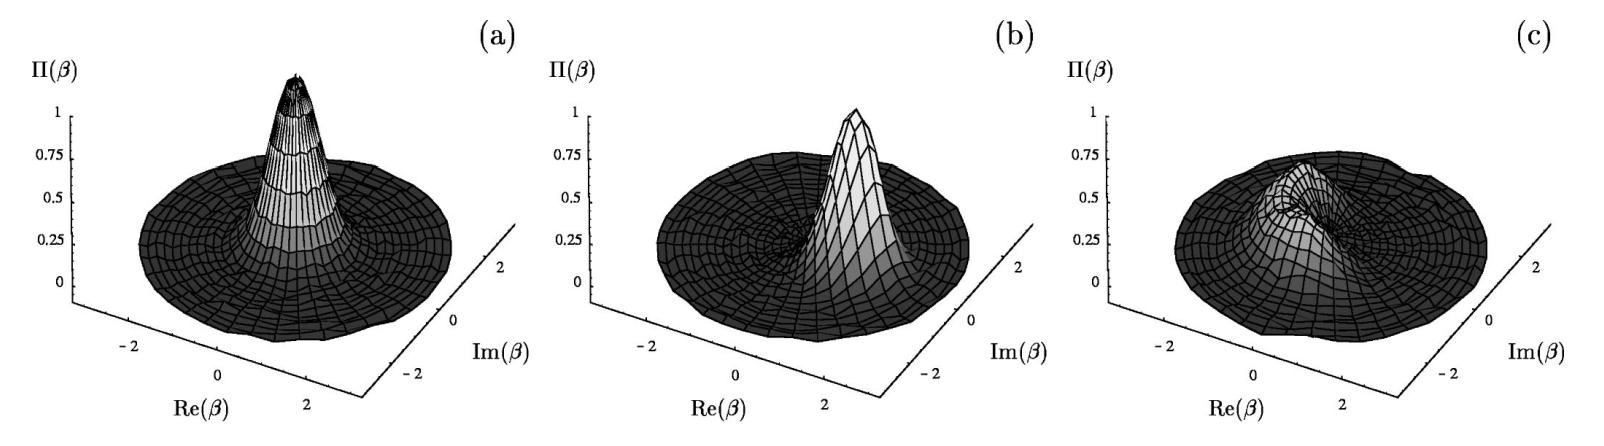
\includegraphics[width=400px,height=111px]{Figures/BanaResults.png}%
\caption{Measured results of three quantum states prepared by Banaszek et. al. Panel a) corresponds to measurements conducted on the vacuum state. Panel b) corresponds to measurements of a weakly displaced vacuum state. Panel c) corresponds to the coherent state whose phase was modulated using the piezoelectric mirror. $\beta=e^{i\theta}\sqrt{n_{vac}}$. Note that $\beta$ is simply a scaled version of $\alpha$.}%
\label{BanaResults}%
\end{figure}

\section{Hofheinz et. al.}
As a small, final example of an experimental determination of the Wigner function of quatnum states, I present the paper of Hofheinz et. al., 2009 \cite{Hofheinz}.

This architecture is different still than the optical platforms already discussed. It involves the use of superconducting circuits. But, the implementation follows the same math, so the results should be the same (excluding environmental differences between the two types of schemes). In not so many words, (because there is not room for many more), microwave pulses are applied to the qubit (see figure \ref{HofheinzSetUp}) to excite the qubit into an arbitrary superposition of $\ket{0}$ and $\ket{1}$. Initially, the qubit transition frequency is detuned (off-resonance) from the resonator frequency. This deters unwanted, spontaneous energy transfer from the qubit to the resonator. Once the state has been prepared in the qubit, the qubit is brought on resonance with the resonator and the exchange of a photon from the qubit to the resonator takes place. By repeatedly doing this and keeping track of the phase of old photons, one can generate arbitrary Fock states in the resonator. Then, the resonator can be probed and analyzed over many instantiations of the state of interest. This allows full tomography to be conducted on the state and the Wigner function to be determined. The results of their measurements are shown in figure \ref{HofheinzResults}.	

\begin{figure}%
\begin{center}
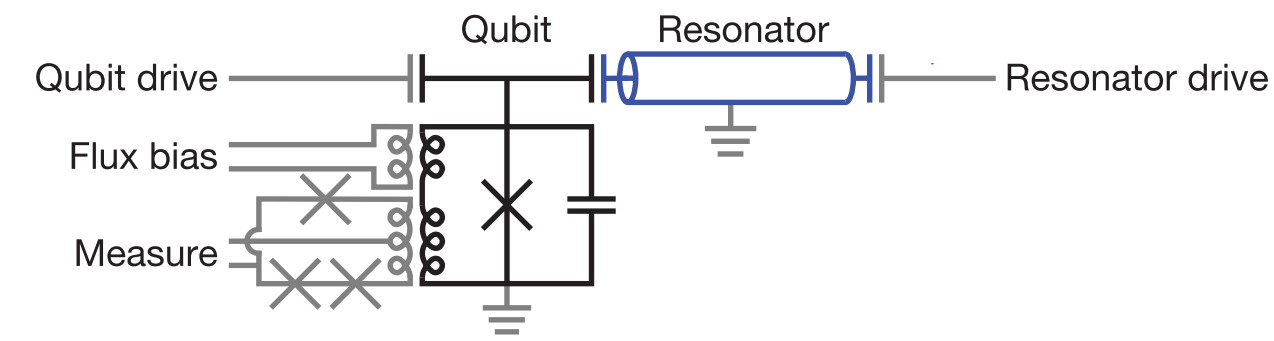
\includegraphics[width=300px,height=80px]{Figures/HofheinzSetUp.png}%
\caption{Circuit schematic of the superconducting circuit used in the Hofheinz et. al. paper of 2009.}%
\label{HofheinzSetUp}%
\end{center}
\end{figure}


\begin{figure}%
\begin{center}	
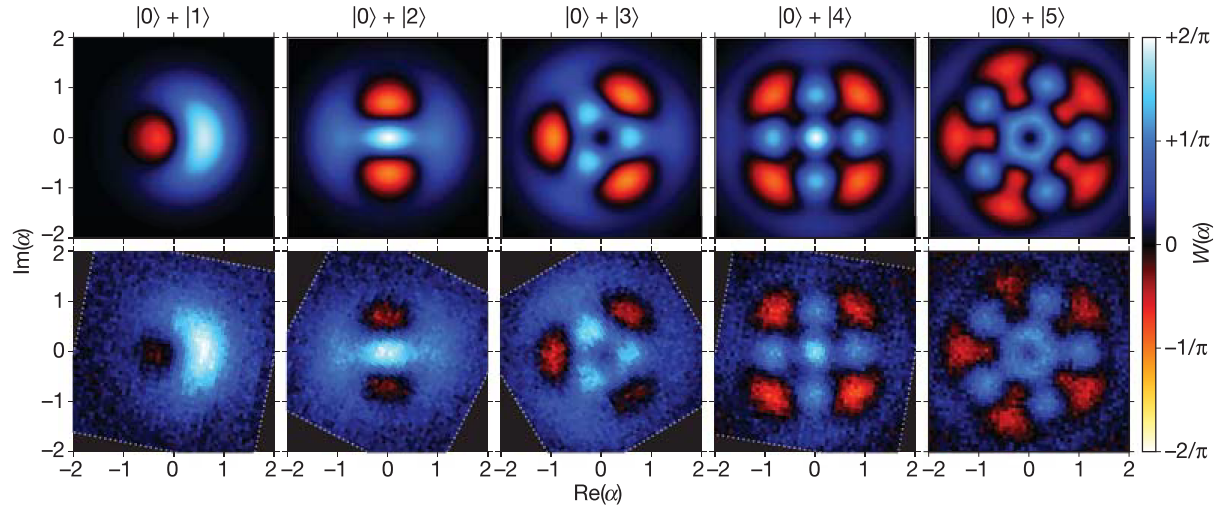
\includegraphics[width=300px,height=125px]{Figures/HofheinzResults.png}%
\caption{Results reported from the 2009 Hofheinz paper.}%
\label{HofheinzResults}%
\end{center}
\end{figure}


\section{Conclusion}
In conclusion, numerous researchers have published papers highlighting the feasibility of quantum state tomography using the Wigner representation of the quantum state. However, all of this being said, Wigner state representations have little experimental relevance. Most quantum computational engineers characterize their states using the density matrix representation, which is equivalent. But, considering the case of a quantum system whose states are continuous under the parameter of interest (like coherent states under the parameter $\alpha$) a density matrix representation may not be as direct as a continuous state-space representation as provided by the Wigner function.

Experimentalism aside, though, Wigner functions have been receiving a lot of attention by theoretical physicists within the last decade in that they lend themselves nicely to understanding how much ``quantum resource'' exists in a certain state \cite{Veitch}.  Coherent states of light (the appropriate description of light in the classical regime) are entirely positive in phase space. Fock states, however, must, and are always, negative over portions of the phase space. This motivates correlating the amount of ``quantum resource'' with the amount of negativity of the state's Wigner representation in phase space. So, while the Wigner representation may not be consistently practical to obtain experimentally, it is theoretically useful and is seeing much use in this domain, today (especially in the field of quantum optics).

\clearpage		
%%%%%%%%%%%%%%%%%%%%%%%%%%%%%%%%%%%%%%%%%%%%%%%%%%%%%%%%%%%%%
%% ==> Some hints are following:

%% <== End of hints
%%%%%%%%%%%%%%%%%%%%%%%%%%%%%%%%%%	 	%%%%%%%%%%%%%%%%%%%%%%%%%%%



%%%%%%%%%%%%%%%%%%%%%%%%%%%%%%%%%%%%%%%%%%%%%%%%%%%%%%%%%%%%%
%% BIBLIOGRAPHY AND OTHER LISTS
%%%%%%%%%%%%%%%%%%%%%%%%%%%%%%%%%%%%%%%%%%%%%%%%%%%%%%%%%%%%%
%% A small distance to the other stuff in the table of contents (toc)

%% The Bibliography
%% ==> You need a file 'literature.bib' for this.
%% ==> You need to run BibTeX for this (Project | Properties... | Uses BibTeX)
%\addcontentsline{toc}{chapter}{Bibliography} %'Bibliography' into toc
%\nocite{*} %Even non-cited BibTeX-Entries will be shown.
\bibliographystyle{plain} %Style of Bibliography: plain / apalike / amsalpha / ...
\bibliography{References} %You need a file 'literature.bib' for this.

%% The List of Figures

%% The List of Tables	

%%%%%%%%%%%%%%%%%%%%%%%%%%%%%%%%%%%%%%%%%%%%%%%%%%%%%%%%%%%%%
%% APPENDICES
%%%%%%%%%%%%%%%%%%%%%%%%%%%%%%%%%%%%%%%%%%%%%%%%%%%%%%%%%%%%%
\appendix
%% ==> Write your text here or include other files.

%\input{FileName} %You need a file 'FileName.tex' for this.
\end{document}

